% !TeX spellcheck = cs_CZ
%{\tikzset{external/prefix={tikz/CES/}}
% \tikzset{external/figure name/.add={ch05_}{}}
%---------------------------------------------------------------------------------------------------
% file ANSI_C_MCU.tex
%---------------------------------------------------------------------------------------------------
%============================= Kapitola: Stručný úvod===============================================
\lstset{ %
  language=C,                            % choose the language of the code
  basicstyle=\footnotesize\ttfamily,     % the size of the fonts that are used for the code
  backgroundcolor=\color{White},         % choose the background color. 
  commentstyle=\color{help}\textit,
  keywordstyle=\color{blue}\textbf,
  breaklines=true,                       % sets automatic line breaking
  breakatwhitespace=true,                % sets if automatic breaks should only happen at whitespace
  showspaces=false,                      % show spaces adding particular underscores
  showstringspaces=true,                 % underline spaces within strings
  showtabs=true,                         % show tabs within strings adding particular underscores
  frame=none,                            % adds a frame around the code - none, single
  tabsize=8,                             % sets default tabsize to 8 spaces
  captionpos=b,                          % sets the caption-position to bottom
  numbers=left,                          % where to put the line-numbers -none, left, right
  numberstyle=\footnotesize,             % the size of the fonts that are used for the line-numbers
  stepnumber=1,                          % the step between two line-numbers. If it's 1 each line
  % will be numbered
  xleftmargin=3em,                       % adjust left margin
}

\chapter{C pro mikrokontroléry}
\minitoc
  \wikiANSIC je programovací jazyk, který počátkem 70. let 20. století vyvinuli Ken Thompson a 
  Dennis Ritchie pro potřeby operačního systému Unix. V současné době je to jeden z 
  nejpopulárnějších jazyků, zřejmě nejčastější pro psaní systémového softwaru, ale velmi rozšířený 
  i pro aplikace. C je nízkoúrovňový, kompilovaný, relativně minimalistický programovací jazyk. Je 
  dostatečně mocný na většinu systémového programování (ovladače a jádro OS), přičemž zbytek lze 
  dořešit tzv. \wikiInlineASM, tedy metodou zápisu assembleru přímo do kódu. Zdrojový kód C je 
  přitom mnohem čitelnější než assembler, je jednodušší ho zapsat a navíc je daleko snáze 
  přenositelný na jiné procesory a počítačové architektury. Proto jsou často operační systémy, 
  překladače, knihovny a interprety vysokoúrovňových jazyků implementovány právě v C. Mnoho dalších 
  moderních programovacích jazyků přebírá způsob zápisu (neboli syntaxi) z jazyka C, například 
  \wikiCPP, Java, Perl a PHP.

  \begin{figure}[ht!]  %\ref{fyz:fig077}
    \centering
    \includegraphics[width=0.5\linewidth]{ces_fig007.jpg}
    \caption{Autoři jazyka C Ken Thompson a Dennis Ritchie přebírají ocenění v podobě Národní 
             medaile za technologii (v roce 1998) od Billa Clintona}
    \label{ces:fig007}
  \end{figure}

  V roce 1973 se stal jazyk C dostatečně stabilním. Většina zdrojového kódu jádra Unixu, původně 
  napsaného v assembleru, byla přepsána do C. Unix tedy patří mezi první operační systémy, které 
  byly napsané v jiném než strojovém jazyce či assembleru. 
  
  \begin{description}
    \item[K\&R C] V roce 1978, Ritchie a Brian Kernighan vydali první vydání knihy \emph{The C 
                  Programming Language}. Tato kniha, mezi programátory C známá jako „K\&R“, 
                  sloužila po mnoho let jako neformální specifikace jazyka. Verze C, kterou takto 
                  popsali, bývá označována jako „\textbf{K\&R C}“. (Druhé vydání knihy popisovalo 
                  novější standard ANSI C.)
    \item[C89]    V roce 1983 se American National Standards Institute (ANSI) dohodla na sestavení 
                  komise, aby vytvořila standardní specifikaci C. Po dlouhém procesu byl standard 
                  dokončen v roce 1989 a schválen jako ANSI X3.159-1989 „\emph{Programming Language 
                  C}“. Tato verze jazyka je často stále označována jako \textbf{ANSI C} nebo 
                \textbf{C89}.
  \end{description}
  

  

  
 
  
  V roce 1990 byl standard ANSI C (s drobnými změnami) adoptován institucí International 
  Organization for Standardization (ISO) jako „ISO 9899|ISO/IEC 9899:1990“. Formálně tak nahradil 
  předchozí verzi C89/ANSI-C a tato revize je označována jako \textbf{C90} neboli \uv{jazyk C},
  
  Po standardizaci jazyka v roce 1989 - 1990 se většina vývoje soustředila na jazyk C++. Přesto 
  však na konci 90. let došlo k vydání dokumentu ISO 9899:1999 (obvykle nazývaný \textbf{C99}), 
  který byl následně v březnu 2000 přijat i jako ANSI standard.
  
  První norma pro C byla tedy vydána společností ANSI. Ačkoli tento dokument byl následně přijat 
  Mezinárodní organizací pro normalizaci (ISO) a následné revize vydané společností ISO byly také 
  přijaty ANSI, mnozí programátoři stále používají "\emph{ANSI C}", ačkoliv se odkazují na ISO 
  standard. Jiní vývojáři softwaru používají termín \emph{ISO C}, ostatní jsou neutrální a 
  používají \emph{Standard C}.
    
  %============= Podkapitola: Konstrukce a struktura programu v jazyce C ===========================
  \section{Konstrukce a struktura programu v jazyce C}
  %============= Podkapitola: Proměnné datové typy, rozsahy platnosti a hodnot =====================
  \section{Proměnné datové typy, rozsahy platnosti a hodnot}
  %============= Podkapitola: Operátory ============================================================
  \section{Operátory}
  %============= Podkapitola: Funkce a práce s pamětí ==============================================
  \section{Operátory}
    \subsection{Bitové  operátory}
      Protože jazyk C je oproti jiným vyšším jazykům zaměřen na přeci jen poněkud nižší úroveň, 
      nabízí programátorům i operátory, pomocí kterých mohou nepřímo pracovat i s jednotlivými bity.
      Tuto možnost zdaleka nemají všechny programovací jazyky označované jako \emph{vyšší}.
      
      Bitové operátory \(<<\), \(>>\), \&, |, \~, \^, tedy posun vlevo, posun vpravo, and, or, not 
      a xor jsou povoleny pouze pro celočíselné (integer) datové typy char, int, short, long (se 
      znaménkem (signed) nebo bez znaménka (unsigned)). V závislosti na MCU a kompilátoru se tyto 
      příkazy převádějí na odpovídající výkonné strojové instrukce. Toto hardwarově blízké bitové 
      řízení často nalézá uplatnění při přístupu na speciální registry v mikrokontroléru. 
      (\cite[s.~79]{Burkhard2003}).
      
      Při bitovém posunu vlevo (vpravo) << , ( >> ) se jednotlivé bity posouvají vlevo (vpravo), 
      tedy do pozice s (binárně) vyšším (nižším) řádem. Na nejpravější (nejlevější) posunem 
      vytvořenou pozici je umístěna nula. Posuny ovšem probíhají aritmeticky. To znamená, že 
      uvedené pravidlo neplatí pro posun vpravo hodnoty celočíselného typu se znaménkem. V takovém 
      případě se nejvyšší bit (znaménkový), zachovává. Takto se při posunu doplňuje do bitového 
      řetězce nový bit. Naopak před posunem nejlevější (nejpravější) bit je odeslán do
      "říše zapomnění.
      
      Bitový posun o jeden (binární) řád vpravo, respektive vlevo, má stejný význam, jako 
      celočíselné dělení, respektive násobení, dvěma. Je-li bitový posun o více než jeden řád, 
      jedná se o násobení (dělění) příslušnou mocninou dvou.
      
      Bitové and \& , or |, a xor \^ provádí příslušnou binární operaci s každým párem 
      odpovídajících si bitů. Výsledek je umístěn do pozice stejného binárního řádu výsledku. 
      Výsledky operací nad jednotlivými bity jsou  stejné, jako v Booleově algebře9. Bitové not \~ 
      je operátorem unárním, provádí negaci každého bitu v bitovém řetězci jediného operandu. 
      Tomuto operátoru se často říká bitový doplněk. 
      
      \subsubsection{Makra pro bitové operace}
        O něco elegantnější je použití maker k nahazování, shazování a testování bitových míst. 
        \lstset{numbers=none}
        \begin{lstlisting}{}
          #define SET_BIT(REG, BIT)     ((REG) |= (BIT))
          #define CLEAR_BIT(REG, BIT)   ((REG) &= ~(BIT))
          #define READ_BIT(REG, BIT)    ((REG) & (BIT))
        \end{lstlisting}
        Takto vypadají makra pro bitové operace: nastav bit, smaž bit, čti bit v knihovně 
        \texttt{STM32F4 Library} (\texttt{stm32f4xx.h})
      
  %============= Podkapitola: Pointery =============================================================
  \section{Pointery}
    \textbf{Pointery} (též ukazatele nebo směrníky) jsou \emph{"srdce a duše jazyka C"}. Pointer je 
    proměnná, jako každá jiná, pouze hodnota uložená v této proměnné má jiný význam. Pointer 
    představuje \textit{adresu paměti} a na této adrese se teprve ukrývá příslušná hodnota. Pointer 
    je tedy proměnná uchovávající paměťovou adresu.\cite{Herout}
  
    \subsection{Práce s pointery}
      \begin{figure}
        \centering
        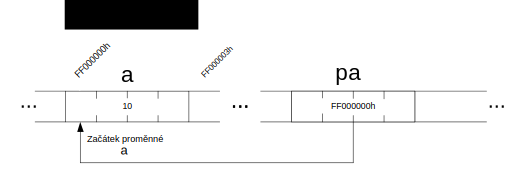
\includegraphics[width=0.9\linewidth]{princip_ukazatele.pdf}
        \caption{Princip ukazatele v paměti}
        \label{figure:pointer1}
      \end{figure}
      \begin{example}Vytvořte funkce kopírující prvky jednoho pole do druhého pomocí indexu i 
      ukazatele.
      
        % \marginpar{\includegraphics[width=0.09\textwidth]{pen.pdf}}
        %---------------------------------------------------------------
        \lstinputlisting[caption=\texttt{CPYARRY.C} Kopíruje prvky jednoho pole do 
          druhého.]{../src/CES/C/CPYARRY.c}
        %---------------------------------------------------------------
        Výstup programu:                                                     \newline
          \lstinline[basicstyle=\ttfamily]!1   2   3   4   5   6   7   8   9!\newline
          \lstinline[basicstyle=\ttfamily]!1   2   3   4   5   6!            \newline
          \lstinline[basicstyle=\ttfamily]!4   5   6   7   8   9!            \newline
      \end{example} 

  %============= Podkapitola: Preprocesor jazyka C =================================================
  \section{Preprocesor jazyka C}
    Preprocesor interpretuje jednoduché direktivy pro vložení zdrojového kódu z jiného souboru 
    (\lstinline[basicstyle=\ttfamily]!#include!), definice maker 
    (\lstinline[basicstyle=\ttfamily]!#define!) a podmíněné vložení kódu 
    (\lstinline[basicstyle=\ttfamily]!#if!). \texttt{C} preprocesor přijímá tyto direktivy:
    
    \begin{table}[ht!]
      \centering
      \begin{tabular}{c c c c}
        \hline
        \lstinline[basicstyle=\ttfamily]!#define!  & \lstinline[basicstyle=\ttfamily]!#elif! & 
        \lstinline[basicstyle=\ttfamily]!#else!    & \lstinline[basicstyle=\ttfamily]!#endif!  \\
        \lstinline[basicstyle=\ttfamily]!#error!   & \lstinline[basicstyle=\ttfamily]!#if! & 
        \lstinline[basicstyle=\ttfamily]!#ifdef!   & \lstinline[basicstyle=\ttfamily]!#ifndef! \\
        \lstinline[basicstyle=\ttfamily]!#include! & \lstinline[basicstyle=\ttfamily]!#line! & 
        \lstinline[basicstyle=\ttfamily]!#pragma!  & \lstinline[basicstyle=\ttfamily]!#undef!  \\
        \hline            
      \end{tabular}
      \caption{Seznam platných direktiv jazyka \texttt{C}}\label{S4101C1:C_tab_direktiva}
    \end{table} 
    
    \subsection{Připojení externích souborů}
    
    \subsection{Definice maker}
      Definice maker ve významu rozsahů polí je typickým příkladem použití preprocesoru. Ve 
      zdrojovém textu se neodvoláváme na magická čísla, ale na vhodně symbolicky pojmenovaná makra, 
      která zvýší čitelnost programu.
      
      Pro větší přehlednost rozdělme makra na 
      \begin{itemize}
       \item symbolické konstanty,
       \item makra
      \end{itemize}
      Klíčem nechť je skutečnost, že makro na rozdíl od symbolické konstanty má argumenty.
      \subsection{Symbolické konstanty}
      \subsection{Makra}
     
    \subsection{Podmíněný překlad}  
      Preprocesor může během své činnosti vyhodnocovat, je-li nějaké makro definováno, či nikoliv. 
      Při použití klíčového slova preprocesoru \texttt{defined} pak může spojovat taková 
      vyhodnocení do rozsáhlejších logických výrazů. Argument defined nemusí být uzavřen do 
      závorek. Může se však vyskytnout jen za \lstinline[basicstyle=\ttfamily]!#if! nebo 
      \lstinline[basicstyle=\ttfamily]!#elif!. Například si ukažme složitější podmínku:


  %============= Podkapitola: Terminálový vstup a výstup============================================
  \section{Terminálový vstup a výstup}
    Jazyk C, narozdíl od Pascalu, nedefinuje žádnou \texttt{I/O (vstup\-ně/výstup\-ní 
    -In\-put/Out\-put)} operaci jako část jazyka. Nezbytné vstupy a výstupy jsou řešeny tak, že 
    standardní knihovna obsahuje několik funkcí, které \texttt{I/O} zajišťují.
  
    Nejvíce strojově závislé akce jsou I/O operace a tímto způsobem se tedy důsledně oddělují 
    strojově závislé a strojově nezávislé části jazyka. Tato skutečnost je pak významným přínosem 
    při vytváření kompilátoru pro jiný počítač.
  
    \begin{figure}[ht!]
      \centering
      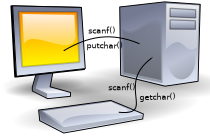
\includegraphics[scale=1.2]{terminalovy_IO_skica.pdf}
      \caption{Operace pro terminálový vstup a výstup}\label{C:fig_Terminal_IO}
    \end{figure}
  
    \subsection{Hlavičkový soubor \texttt{stdio.h}}
      Aby bylo možno správně používat všechny funkce pro vstupu a výstupu, je nutné na začátku 
      programu připojit "popis" těchto funkcí. Ten se nachází v hlavičkovém (\emph{header}) souboru 
      \lstinline[basicstyle=\ttfamily]!stdio.h!:
  
      \lstinline[basicstyle=\ttfamily]!#include <stdio.h>  //zde neni strednik!
  
      Od tohoto okamžiku je pak možné používat dále popsané funkce.
  
    \subsection{Standardní vstup a výstup znaku}
      Výstup jednoho znaku zajišťuje \lstinline[basicstyle=\ttfamily]!putchar()! a vstup jednoho 
      znaku funkce \lstinline[basicstyle=\ttfamily]!getchar()!.
      \begin{itemize}
        \item \lstinline[basicstyle=\ttfamily]!int putchar(int c);!
        \item \lstinline[basicstyle=\ttfamily]!int getchar(void);!
      \end{itemize}
      Obě funkce pracují s proměnnými \lstinline[basicstyle=\ttfamily]!int! a ne 
      \lstinline[basicstyle=\ttfamily]!char!.
  
        % \marginpar{\includegraphics[width=0.09\textwidth]{pen.pdf}}
        %---------------------------------------------------------------
        \lstinputlisting[caption=\texttt{Cteni\_tisk\_znaku.c} Čtení a tisk znak ze 
           standardního vstupu na standardní výstup.]{../src/CES/C/Cteni_tisk_znaku.c} 
        %--------------------------------------------------------------    
      
      \begin{example}Čtení znaku ze standardního vstupu a jejich zápis na standardní výstup 
        ukazuje následující program, představující jednoduchou variantu příkazu kopírování souboru 
        (nutno ovšem přesměrovat vstup a výstup).
  
        % \marginpar{\includegraphics[width=0.09\textwidth]{pen.pdf}}
        %---------------------------------------------------------------
        \lstinputlisting[caption=\texttt{CPY.c} Kopíruje znak ze standardního vstupu na 
                standardní výstup.]{../src/CES/C/CPY.c}
        %---------------------------------------------------------------
      \end{example}
      
    \subsection{Standardní vstup a výstup řetězců}
      Standardní vstup a výstup řetězců je jednoduchou nadstavbou nad čtením znaku. Obě funkce,
      \begin{itemize}
        \item \lstinline[basicstyle=\ttfamily]!char *gets(char *s);!
        \item \lstinline[basicstyle=\ttfamily]!int puts(const char *s);!
      \end{itemize}
      pracují s řetězci. \texttt{gets()} načte do znakového pole vstupní řetězec az do konce řádku, 
      symbol  \lstinline[basicstyle=\ttfamily]!'\n'! není do znakového pole zapsán. Ukazatel na 
      pole (načtený řetězec) je rovněž návratovou hodnotou. Chybu signalizuje návrat NULL. 
      \texttt{puts()} 
      zapíše řetězec na výstup a přidá přechod na novy řádek       
      \lstinline[basicstyle=\ttfamily]!'\n'!. Chybu představuje návratové \texttt{EOF}, jinak vrací 
      kladné cele číslo.
  
      Jednoduchost použití skrývá velké nebezpečí. Funkce \texttt{gets()} nemá informaci o délce 
      oblasti vymezené pro čtený řetězec. Je-li oblast kratší, než vstupní řádek, dojde jeho 
      načtením velmi pravděpodobně k přepsání paměťové oblasti související s vyhrazenou pamětí. A 
      to se všemi důsledky z toho vyplývajícími.
  
    \subsection{Formátovaný standardní vstup a vystup}
    \subsection{Souhrnné cvičení}
      \begin{example}Vytvořte program, který vygeneruje ASCII tabulku se čtyřmi sloupci ve formátu 
      \textbf{[znak|kód|znak|kód]}. Rozsah tabulky definujte pomocí dvou symbolických konstant 
      \lstinline[basicstyle=\ttfamily]!MIN_ASCII, MAX_ASCII!. 
  
        % \marginpar{\includegraphics[width=0.09\textwidth]{pen.pdf}}
        %---------------------------------------------------------------
        \lstinputlisting[caption=\texttt{ASCII.c} Generuje ASCII tabulku na terminálu.]{../src/CES/C/ASCII.c}
        %---------------------------------------------------------------
      \end{example} 

%} % tikzset
%---------------------------------------------------------------------------------------------------
\printbibliography[title={Seznam literatury}, heading=subbibliography]
\addcontentsline{toc}{section}{Seznam literatury}